\section{Language Integrated Query (LINQ)}
LINQ erlaubt eine Query Syntax um Abfragen an beliebigen Datenstrukturen zu machen. Man unterscheidet den Extension- und Query Expression Syntax (Erinnert an SQL), wobei beide die gleichen Dinge erlauben. Auch LINQ ist reines Compiler Feature.

LINQ kann beliebige Collections durchsuchen, die \lstinline{IEnumerable<>} implementieren. LINQ kennt zwei verschiedene Syntaxen: LINQ Query syntax und die LINQ Method syntax. Der Compiler wandelt Query Expressions in Lambda Expressions (Aufruf der Extension Methods) um.



\begin{itemize}
	\itemsep -0.5em 
	\item Reine Compiler-Technologie
	\item Query-Syntax (ähnlich SQL)
	\item Beliebige Datenstrukturen als Basis (Objekte, XML etc.)
	\item Typensicherheit
	\item Erlaubt funktionale Progammierung mit Lambda
	\item Erlaubt deklarativen Progammierstil mittels Anonymous Types" und Object "initializers"
	\item Verbesserung Type Inference
\end{itemize}

\begin{figure}[h!]
	\centering
	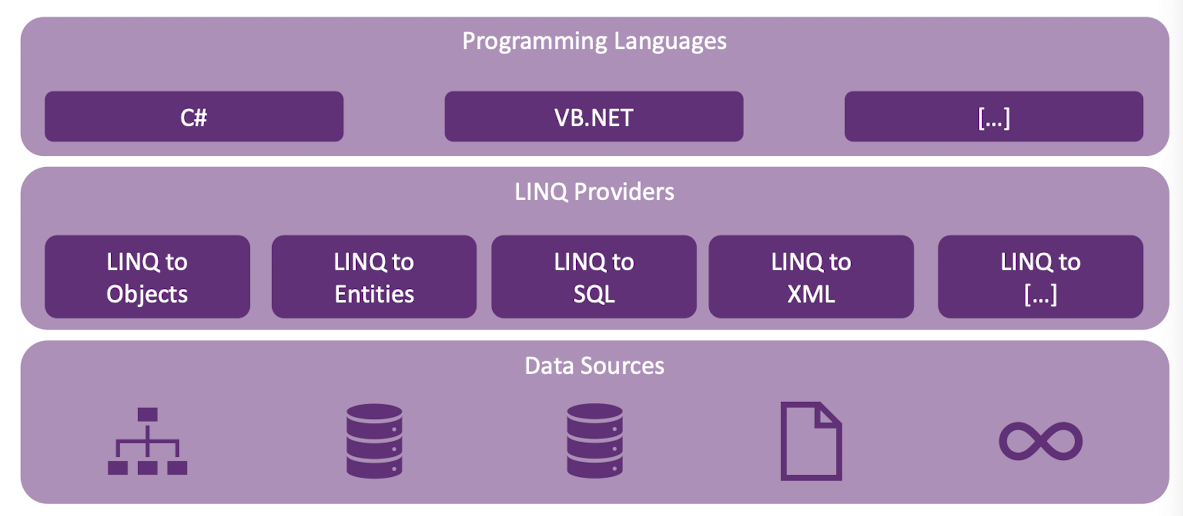
\includegraphics[width=0.5\linewidth]{linq}
  \caption{Compilerumwandlung zu Extension Methods}
\end{figure}

\begin{lstlisting}
// Sequenz				Elemente
string[] name = { "Tom", "Dick", "Harry"};
\end{lstlisting}

\begin{lstlisting}
// Query Expression syntax
var queryWashingtonSorted =
    from e in employees
    where e.State == "WA"
    orderby e.Name descending
    select new
    { e.Name, e.Address };
// Query Extension Method / Lambda syntax
queryWashingtonSorted = employees
    .Where(e => e.State == "WA")
    .OrderByDescending(e => e.Name)
    .Select(e => new
    { e.Name, e.Address });
\end{lstlisting}

\subsection{LINX Extension Methods}
LINQ definiert in der Klasse Enumerable \lstinline{using System.Linq;} eine Vielzahl von Query Operatoren. Die Methoden in dieser Klasse stellen eine Implementierung von Operatoren zum Abfragen von Datenquellen bereit, die \lstinline{IEnumerable<T>} implementieren.

\begin{lstlisting}
int[] numbers = { 1, 4, 2, 9, 13, 8, 9, 0, -6, 12 };
IEnumerable<int> res = numbers
	.Where(i => i >= 5) 
	.OrderBy(i => i);
IEnumerable<int> sqr = numbers
	.Skip(2) 
	.Take(4) 
	.Select(k=> k * k);

\end{lstlisting} 

\subsection{Expression-Bodies Members}
Ermöglichen uns in einer kurz gehaltenen Syntax Methoden und Properties zu definieren. Dies erlaubt es uns den return sowie den body wegzulassen.

\begin{lstlisting}
public class Examples {
private int value;
	// Constructors / Destructors (C# 7.0) 
	public Examples(int v) => this.value = v;
	~Examples() => this.value = 0;
	// Methods (C# 6.0) 
	public int Sum(int x, int y) => x + y;
	
	public int GetZero() => 0; 
	public void Print() => Console.WriteLine("...");
	// Properties (C# 6.0) 
	public int Zero => 0; 
	public int Bla => Sum(Zero, 2);
	// Getters/Setters (C# 7.0) 
	public int Value {
		get => this.value; 
		set => this.value = value;
	}
}
\end{lstlisting}

\subsection{Query Expressions Synax}
\begin{lstlisting}
// 1. Datenquelle waehlen
int[]numbers={0,1,2,3,4,5,6};

// 2. Query erstellen
var numQuery = from num in numbers 
	where (num % 2) == 0
	select num;

// 3. Query ausfuehren
foreach (int num in numQuery) { Console.Write("{0,1} ", num); }	
\end{lstlisting}

\begin{itemize}
  \itemsep -0.5em 
  \item from: Datenquelle
  \item where: filter
  \item orderby: Sortierung
  \item select: Projektion
  \item group: Gruppierung ein eine Sequenz von Gruppen Elementen
  \item join: Verknüpfung zweier Datenquellen
  \item let: definition von Hilfsvariablen
\end{itemize}

\begin{figure}[h!]
  \center
  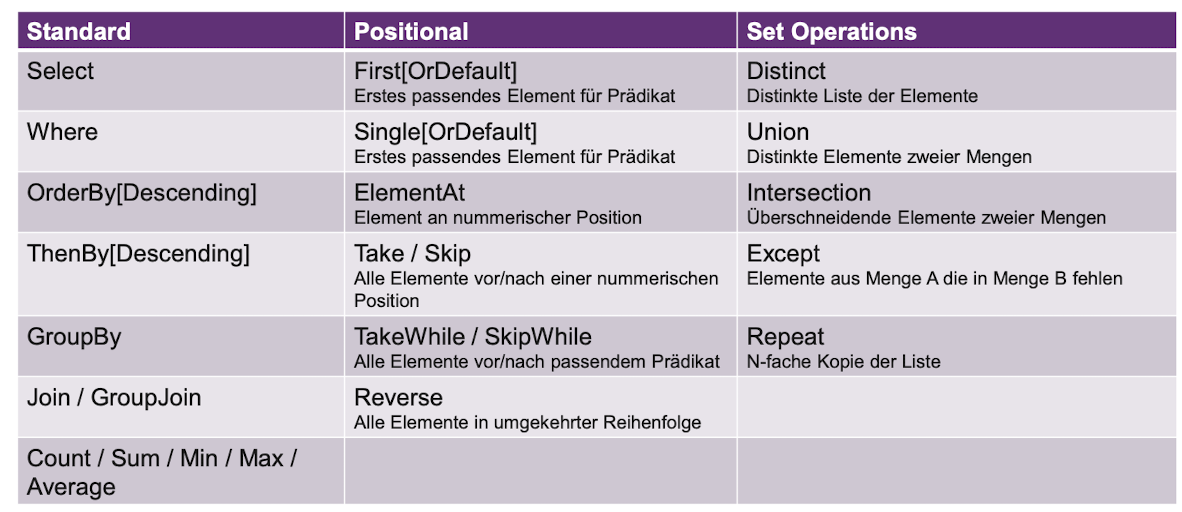
\includegraphics[width=0.75\linewidth]{queryexpressions}
  \caption{Query Operatoren / Extension Methoden}
\end{figure}

\subsection{Gruppierung}
\begin{lstlisting}
// q: IEnumerable<IGrouping<string, string>> 
var q = from s in Students
	group s.Name by s.Subject;
} 

// Gruppierung mit direkter Wiederverwendung
var q = from s in Students
	group s.Name by s.Subject into g 
	select new {
      Field = g.Key,
      N = g.Count()
   };

// Anz. Bestellungen pro Datum
from best in Bestellungen
group best by best.Datum into datumGroup 
orderby datumGroup.Key
select new {
   Datum = datumGroup.Key,
   Anzahl = datumGroup.Count()
};
\end{lstlisting}

\subsection{Inner Joins}
Ein Inner Join nimmt nur jene Ergebnisse, die nicht null sind.
\begin{lstlisting}
var q = from s in Students
	join m in Markings on s.Id equals m.StudentId 
	select s.Name + ", " + m.Course + ", " + m.Mark
\end{lstlisting}

\subsection{Group Joins}
Ein Group Join verwendet die into Expression.
\begin{lstlisting}
var q = 
	from s in Students 
	join m in Markings on s.Id equals m.StudentId
		into list
	select new
      Name = s.Name,
      Marks = list
	};
\end{lstlisting}

\subsection{Left Outer Joins}
\begin{lstlisting}
var q = from s in Students
	join m in Markings on s.Id equals m.StudentId into match 
	from sm in match.DefaultIfEmpty()
	select s.Name + ", " + (sm == null
      ? "?"
      : sm.Course + ", " + sm.Mark);	
\end{lstlisting}

\subsection{Select Many}
Erleichtert das Zusammenfassen verschachtelter Listen.
%TODO addd select many
\begin{lstlisting}

\end{lstlisting}

\pagebreak
\section{Direct Initialization}
\subsection{Object Initializers}
Object Initialisierer erlaubt das Instanzieren und Initialisieren einer Klasse in einem einzigen Statement. Die Objekte lassen sich auch erzeugen, wenn kein passender Konstruktor zur Verfügung steht.

\begin{lstlisting}
Student s1 = new Student("John") {
	Id = 2009001, // Set public field 
	Subject = "Computing" // Set property
}; 
Student s2 = new Student {
	Name = "Ann", 
	Id = 2009002, 
	Subject = "Mathematics"
};
\end{lstlisting}


\subsection{Collection Initializers}
Ist das selbe wie Objekte Initializers, jedoch mit Listen.

\begin{lstlisting}
List<int> l1 = new List<int> { 1, 2, 3, 4 }; 
Dictionary<int, string> d1 = new Dictionary<int, string>
	{1,"a"}, 
	{2,"b"}, 
	{3,"c"}
};
d1 = new Dictionary<int, string> { 
	[1] = "a",
	[2] = "b",
	[3] = "c"
};

object s = new Dictionary<int, Student> {
	{ 2009001, new Student("John") { 
		Id = 2009001,
		Subject = "Computing" } },
	{ 2009002, new Student {
    	Name = "Ann", Id = 2009002,
        Subject = "Mathematics" } }
};
\end{lstlisting}

\subsection{Anonymous Types (Let)}
\begin{itemize}
  \itemsep -0.5em 
  \item Mit dem Schlüsselwort let wird der Typ vom Compiler herausgefunden
  \item  let kann nur für lokale Variablen verwendet werden. Der Einsatz bei Parametern, Klassenvariablem und Properties ist nicht erlaubt.
  \item Der Typ wird aus der Zuweisung abgeleitet, wobei die Variable zu 100\% typensicher bleibt.
\end{itemize}


\pagebreak
